%! TEX program = xelatex

\documentclass[a4paper,titlepage,UTF8]{ctexbook}

% 导言区
% 包
\usepackage{xeCJK} % 导入中文支持包
\usepackage[colorlinks, linkcolor=blue]{hyperref} % 超链接的颜色设置为红色
\usepackage{xcolor}
\usepackage{listings}
\usepackage{geometry}
\usepackage{fancyhdr}
\usepackage{cite}
\usepackage[super]{gbt7714} % 中文文献包
\usepackage{graphicx} % 导入图片包
\graphicspath{{img/game/},{img/install/},{img/screenfetch/}}
\usepackage{subfig}
\usepackage{tabularx}
\usepackage{chngpage}
\usepackage{array}
\usepackage{parskip}
\usepackage{booktabs}

\newfontfamily\consolas{Consolas}

% green
\definecolor{mygreen}{rgb}{0, 0.6, 0}

% 页边距
\geometry{left=2.5cm,right=2.5cm,top=2.0cm,bottom=2cm}

% 页眉页脚
\pagestyle{empty}

\lstset{
	basicstyle=\small\consolas,
	numberstyle= \tiny, 
	keywordstyle= \color{ blue!70},
	commentstyle=\color{mygreen},
	frame=shadowbox, 
	rulesepcolor= \color{ red!20!green!20!blue!20},
	columns=flexible, % 等宽字体
} 

% 中文设置
\setCJKmainfont{思源宋体}

% 英文设置
\setmainfont{JetBrains Mono}

% 标题页
\title{Qt中文文档翻译}
\author{作者:\href{https://github.com/QtDocumentCN}{QtDocumentCN}}
\CTEXoptions[today=small]
 % 标题左对齐
\CTEXsetup[format={\Large}]{section}

% 首行缩进两个字符
%\setlength{\parindent}{2em}

\begin{document}
% 正文区(文稿区)
% 页眉页脚
\pagestyle{fancy}
\lhead{
\includegraphics[scale=0.1]{./img/logo.png}}
\renewcommand{\headrulewidth}{0.4pt}

\maketitle
\tableofcontents
\thispagestyle{empty} % 目录页不显示页码
%\chapter{贡献}
\begin{figure}[hbt!]
	\centering
	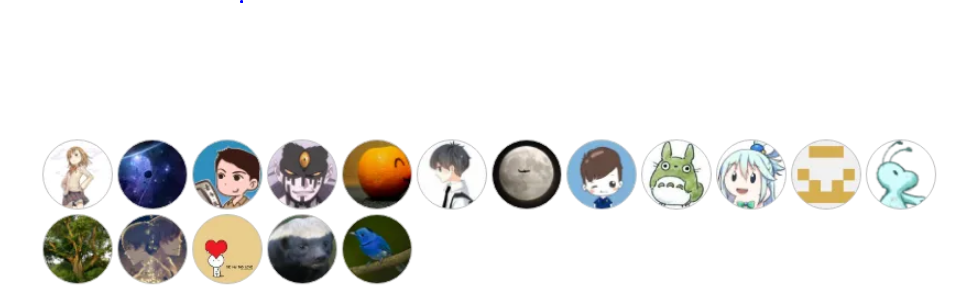
\includegraphics[width=\textwidth]{img/Contributors}
\end{figure}
\chapter{参与翻译的人员}

%github 账号 
%翻译的章节
%源文件名

\centering
\begin{tabular}{lll}
	\toprule
	\cmidrule{1-3}
	 Github账号 & 翻译的章节 & 源文件名 \\
	\midrule
	\href{https://github.com/CryFeiFei}{CryFeiFei} & QAbstractAudioOutput & A/QAbstractAudioOutput.tex  \\
	 & QAbstractAnimation & A/QAbstractAnimation.tex  \\
	\href{https://github.com/FlyWM}{FlyWM}  & TODO & TODO.tex \\
	\href{https://github.com/chenjiqing}{chenjiqing}  & TODO & TODO.tex \\	
	\href{https://github.com/skykeyjoker}{skykeyjoker}  & TODO & TODO.tex \\	
	\href{https://github.com/xyz1001}{xyz1001}  & TODO & TODO.tex \\	
	\href{https://github.com/leytou}{leytou}  & TODO & TODO.tex \\	
	\href{https://github.com/froser}{froser}  & TODO & TODO.tex \\	
	\href{https://github.com/chenyanzz}{顾晓}  & TODO & TODO.tex \\
    \href{https://github.com/abc881858}{吴冬亮}  & TODO & TODO.tex \\	
    \href{https://github.com/ZgblKylin}{ZgblKylin}  & TODO & TODO.tex \\	
	\href{https://github.com/JackLovel}{JackLovel}  & TODO & TODO.tex \\
	\bottomrule
\end{tabular}


\chapter{API Design Principles}

API 设计规范

\begin{quote}
译者注:

本文不来自于 Qt 文档,而是来自于 Qt Wiki:\href{https://wiki.qt.io/API_Design_Principles}{API\_Design\_Principles}

API(Application Programming Interface),应用开发接口,本文中也将 P 解释为 Programmer(开发者)。	
\end{quote}

Qt 最出名的特点之一是一致性强、易于学习、功能强大的 API。本文尝试对我们在设计 Qt 风格的 API 中积累的诀窍进行总结。其中许多准则都是通用的,其它的则是习惯性用法,我们主要为了保持接口一致性而继续遵循。

尽管这些准则主要面向公共接口,但也鼓励您在设计内部接口时使用相同的技术,这对与您合作开发的同僚会更加友好。

您可能也会有兴趣查阅 Jasmin Blanchette 的 
\href{https://people.mpi-inf.mpg.de/~jblanche/api-design.pdf}{Little Manual of API Design (PDF)},或它的前身,由 Matthias Ettrich 编写的 \href{https://doc.qt.io/archives/qq/qq13-apis.html}{Designing Qt-Style C++ APIs} 。

优秀接口的六大特点

API 是面向开发者的,而 GUI 则是面向终端用户。API 中的 P 代表开发者(Programmer),而非程序(Program),目的是指出 API 由开发者,即人类(而非计算机)所使用这一特点。

Matthias 在 Qt 季刊弟13期,关于 API 设计的文章中,声称他坚信 API 应该是最小化但完备的,具备清晰而简洁的语义,符合直觉,被开发者,易于记忆,能够引导开发者编写高可读性的代码。

最小化

最小化的 API 指包含尽可能少的公共成员和最少的类。这可让 API 更易于理解、记忆、调试和修改。

完备性
完备的 API 意味着具备所有应有的功能。这可能会与最小化产生冲突。此外,若一个成员函数位于错误的类中,则大多数潜在的用户回无法找到它。

清晰简洁的语义

与其它设计协作时,应该让您的设计做到最小例外。通用化会让事情更简单。特例可能存在,但不应成为关注的焦点。在处理特定问题时,不应让解决方案过度泛化。(例如,Qt 3 中的 QMineSourceFactory 本该被称作 QImageLoader,并且具备另一套 API。)

复合直觉

如同计算机上其它内容,API 应复合直觉。不同的开发经验和技术背景会导致对复合直觉与否有不同的感知。复合直觉的 API 应能让中等经验的开发者无需阅读文档并直接使用,并让不知道这个 API 的开发者可以理解使用它编写的代码。

易于记忆

为了让 API 易于记忆,请选择一组保持一致并足够精确的命名约定。使用可理解的模式和概念,并且避免缩写。

可读性导向

编写代码只需要一次,但阅读(以及调试和修改)则会非常频繁。高可读性的代码通常需要花更多时间编写,但可以在产品的生命周期中节约更多的时间。

最后需要谨记,不同类型的用户会使用 API 的不同部分。在单纯地创建一个 Qt 类实例能非常直观的同时,希望用户在尝试继承它之前先阅读文档则是很合理的。

静态多态

相似的代码类应具有相似的 API。可以使用继承来实现——当运行时多态支持时,这是很合理的。但多态同时也可以体现在设计截断。例如,若将代码中的 QProgressBar 换为 QSlider,或将 QString 换为 QByteArray,他们间相似的 API 会另替换操作变得非常容易。这便是为何我们称之为“静态多态”。

静态多态同样可让记忆 API 和开发模式变得更加简单。结果是,对于一组有关联的类,相似的 API 通常比为每个类独立设计的完美 API 更加好用。

在 Qt 中,当不具备有足够说服力的原因时,我们更倾向于使用静态多态,而非继承。这减少了 Qt 的公共类数量,并让新用户更容易在文档中找到需要的内容。

好的

​ QDialogBox 和 QMessageBox 具有相似的 APi,以用于处理按钮(addButton(), setStandardButtons(),但无需继承自某些 "QAbstractButtonBox" 类。

坏的

​ QAbstractSocket 被 QTcpSOcket 和 QUdpSocket 所继承,但这两个类的交互方式差异很大。看起来并没有人使用过(或能够使用) QAbstractSocket 指针来进行通用且有效的操作。

存疑

​ QBoxLayout 是 QHBoxLayout 和 QVBoxLayout 的基类。优点:可以在工具栏中使用 QBoxLayout,调用 setOrientation() 来令其水平/垂直排布。缺点:引入额外的类,用户可能会写出形如 ((QBoxLayout *)hbox)->setOrientation(Qt::Vertical) 的代码,而这是不合理的。

基于属性的 API
比较新的 Qt 类倾向于使用基于属性的 API,例如:

\begin{lstlisting}
QTimer timer;
timer.setInterval(1000);
timer.setSingleShot(true);
timer.start(); 
\end{lstlisting}

此处的属性,指的是作为对象状态一部分的任何概念性的特征——无论是否是实际的 Q\_PROPERTY。只要可行,用户都应该允许以任何顺序设置属性,也就是说,这些属性应该是正交的。例如,上文的代码也可以写为:

\begin{lstlisting}
QTimer timer;
timer.setSingleShot(true);
timer.setInterval(1000);
timer.start(); 
\end{lstlisting}

为了方便,我们也可以这样写:

\begin{lstlisting}
timer.start(1000);
\end{lstlisting}

类似的,对于 QRegExp,我们可以:

\begin{lstlisting}
QRegExp regExp;
regExp.setCaseSensitive(Qt::CaseInsensitive);
regExp.setPattern(".");
regExp.setPatternSyntax(Qt::WildcardSyntax);
\end{lstlisting}

为了实现此类 API,内部的对象需要被惰性构造。例如在 QRegExp 的案例中,不应该在还不知道表达式使用何种语法之前,就在 setPattern() 中过早地编译 . 表达式。

属性通常是级联的,此时我们应该谨慎地处理。仔细考虑下当前样式提供的“默认图标大小”与 QToolButton 的 iconSize 属性:

\begin{lstlisting}
toolButton->iconSize(); // 返回当前样式表的默认大小
toolButton->setStyle(otherStyle);
toolButton->iconSize(); // 返回 otherStyle 的默认大小
toolButton->setIconSize(QSize(52, 52));
toolButton->iconSize(); // 返回 (52, 52)
toolButton->setStyle(yetAnotherStyle);
toolButton->iconSize(); // 返回 (52, 52) 
\end{lstlisting}


注意,一旦 iconSize 被设置,它会被一直留存,此时修改当前样式不会影响它。这是 好的。有时,提供重置属性的渠道会很方便,这有两种实现方式:

\begin{itemize}
	\item 传递一个特定值(如 QSIze()、-1 或 Qt::Alignment(0))来指代“重置”;
	\item 提供显示的 resetFoo() 或 unsetFoo() 函数。
\end{itemize}

对于 iconSize,将 QSize()(即 QSize(-1, -1))设为“重置”便足够了。

某些场景中,取值方法会返回值会与设置的内容不同。例如,若调用 widget->setEnabled(true),可能通过 widget->isEnabled() 获得的依然是 false,因为父控件被禁用了。这并没问题,因为通常这正是我们要检查的状态(父控件被禁用时,子控件也应该变灰,表现为也被禁用,但同时在它内部,应该知道自己实际是“可用”的,并等待父控件可用后恢复状态),但必须在文档中正确地进行描述。

QProperty

\begin{quote}
译者注:该类型为 Qt 6.0 引入,需要参见 Qt 6 类文档。

本文原文中的内容与现有的 Qt 6.0 预览版存在出入,因此暂不翻译本节,待官方进一步维护更新原文。
\end{quote}

C++ 特性

值 与 对象

\begin{quote}
译者注:此条原文无内容,待官方更新
\end{quote}

指针 与 引用

作为输出参数,指针与引用哪个更好?

\begin{lstlisting}
void getHsv(int *h, int *s, int *v) const void getHsv(int &h, int &s, int &v) const
\end{lstlisting}

绝大多数 C++ 数据都推荐尽可能使用引用,因为引用在感知上比指针“更安全更漂亮”。事实上,我们在 Qt 软件中更倾向于使用指针,因为这会令代码更加已读。如对比:

\begin{lstlisting}
color.getHsv(&h, &s, &v);
color.getHsv(h, s, v);
\end{lstlisting}

第一行代码能很清晰地表示,h、s、v 对象有很大概率会被该函数调用所修改。

即便如此,由于编译器并不喜欢输出参数,在新 APi 中应该避免此用法,而是返回一个小结构体:

\begin{lstlisting}
struct Hsv { int hue, saturation, value }; Hsv getHsv() const;
\end{lstlisting}

\begin{quote}
	译者注:对于可能失败的带返回值的函数,Qt 倾向于返回数值,使用 bool* ok = 0 参数来存储调用结果,以便在不关心时忽略之。同样在 Qt 6 以后,该方式不再被建议使用,而是改用 std::optional<T> 返回类型。
\end{quote}

传递常引用 与 传递值
若类型大于16字节,传递常引用。

若类型具有非平凡的拷贝构造函数或非平凡的析构函数,传递常引用来避免执行这些方法。

所有其它类型都应使用值传递。

范例:

\begin{lstlisting}
void setAge(int age);
void setCategory(QChar cat);
void setName(QLatin1String name);
void setAlarm(const QSharedPointer<Alarm> &alarm); // 常引用远快于拷贝构造和析构
// QDate, QTime, QPoint, QPointF, QSize, QSizeF, QRect 都是其它应该值传递的好例子
\end{lstlisting}

虚函数

当 C++ 中的一个成员函数被声明为虚函数,这主要用于通过在子类中重写来自定义该函数的行为。将函数设为虚函数的目的是让对该函数的现有调用会被替代为访问自定义的代码分支。若在该类之外没人调用此函数,则在将其声明为虚函数之前需要小心斟酌:

\begin{lstlisting}
// Qt 3 中的 QTextEdit: 成员函数不需要作为虚函数的成员函数
virtual void resetFormat();
virtual void setUndoDepth( int d );
virtual void setFormat( QTextFormat &f, int flags );
virtual void ensureCursorVisible();
virtual void placeCursor( const QPoint &pos;, QTextCursorc = 0 );
virtual void moveCursor( CursorAction action, bool select );
virtual void doKeyboardAction( KeyboardAction action );
virtual void removeSelectedText( int selNum = 0 );
virtual void removeSelection( int selNum = 0 );
virtual void setCurrentFont( const QFont &f );
virtual void setOverwriteMode( bool b ) { overWrite = b; }
\end{lstlisting}




\chapter{QAbstractAnimation}

QAbstractAnimation 是所有的动画相关的基类。

QAbstractAnimation 定义了所有动画类相关的基础功能,通过继承该类,您可以实现动画的其它功能,或者添加自定义的特效。

\begin{tabular}{|r|l|}
	\hline
	属性 & 方法 \\
	\hline
	头文件 & \#include <QAbstractAnimation>\\      
	\hline
	qmake & QT+=core\\      
	\hline
	自从 & Qt 4.6\\
	\hline
	继承&QObject \\
	\hline
	派生 & QAnimationGroup,QPauseAnimation,QVariantAnimation \\
	\hline
\end{tabular}

\section{公共成员类型}

\begin{tabular}{|r|l|}
	\hline
	类型 & 方法 \\
	\hline
	enum & DeletionPolicy \{ KeepWhenStopped, DeleteWhenStopped \}\\      
	\hline
	enum & Direction \{ Forward, Backward \}\\      
	\hline
	enum & State \{ Stopped, Paused, Running \}\\
	\hline
\end{tabular}

\section{属性}

\begin{tabular}{|l|l|l|l|}
	\hline
	属性 & 类型 &属性 &类型 \\
	\hline
		currentLoop & const int &duration &const int \\
	\hline
	currentTime	&int&	loopCount&	int\\
	\hline
	direction	&Direction	&state&	const State\\
	\hline
\end{tabular}


\section{公共成员函数}

\begin{tabular}{|r|l|}

\hline
返回类型 &	函数名\\
\hline
& QAbstractAnimation(QObject *parent = Q\_NULLPTR)\\
\hline
virtual&$\sim$QAbstractAnimation()\\
\hline
int	& currentLoop() const\\
\hline
int	& currentLoopTime() const\\
\hline
int	& currentTime() const\\
\hline
Direction& direction() const\\
\hline
virtual int	&duration() const = 0\\
\hline
QAnimationGroup *&	group() const\\
\hline
int	&loopCount() const\\
\hline
void&	setDirection(Direction direction)\\
\hline
void&	setLoopCount(int loopCount)\\
\hline
State&	state() const\\
\hline
int	& totalDuration() const\\
\hline
\end{tabular}

\section{公共槽}

\begin{tabular}{|r|l|}
\hline
返回类型&	函数名 \\
\hline
void&	pause()\\
\hline
void&	resume()\\
\hline
void&	setCurrentTime(int msecs)\\
\hline
void&	setPaused(bool paused)\\
\hline
void&	start(QAbstractAnimation::DeletionPolicy policy = KeepWhenStopped)\\
\hline
void&	stop() \\
\hline
\end{tabular}



%%% Local Variables:
%%% mode: latex
%%% TeX-master: "../../master"
%%% End:

\chapter{QSql}

QSql 命名空间 里的 各种名样的标识符,已经被运用在 Qt SQL 各个模块中。\href{https://doc.qt.io/qt-5/qsql.html#details}{更多} 

\begin{tabular}{|c|c|p{1.5cm}|}
	\hline
	属性 & 方法 \\
	\hline
	头文件 & \#include <QSql>\\      
	\hline
	qmake & QT += sql\\      
	\hline
\end{tabular}

\section{类型}

\resizebox{\textwidth}{!}{ % Latex表格宽度超出文本宽度
	\begin{tabular}{|c|l|}
		\hline
		&  \\
		\hline
		enum & Location \{ BeforeFirstRow, AfterLastRow \}\\      
		\hline
		enum & NumericalPrecisionPolicy \{ LowPrecisionInt32, LowPrecisionInt64,LowPrecisionDouble,HighPrecision\}\\      
		\hline
		flags & ParamType \\
		\hline 
		enum & ParamTypeFlag \{ In, Out, InOut, Binary \} \\ 
		\hline
		enum & TableType \{ Tables, SystemTables, Views, AllTables \}\\
		\hline
	\end{tabular}
}

细节的介绍 

查看 \href{https://doc.qt.io/qt-5/qtsql-index.html}{Qt SQL}

\section{类型 文档}

enum QSql::Location


此枚举类型描述特殊的sql导航位置


\begin{tabular}{|c|c|c|}
	\hline
	常量	& 值 & 介绍 \\
	\hline
	QSql::BeforeFirstRow&-1&在第一个记录之前\\
	\hline
	QSql::AfterLastRow&-2&在最后一个记录之后\\
	\hline
\end{tabular}

\begin{seeAlso}
\href{https://doc.qt.io/qt-5/qsqlquery.html#at}{QSqlQuery::at()}
\end{seeAlso}

enum QSql::NumericalPrecisionPolicy


数据库中的数值可以比它们对应的C++类型更精确。此枚举列出在应用程序中表示此类值的策略。


\resizebox{\textwidth}{!}{ % Latex表格宽度超出文本宽度
	\begin{tabular}{|c|c|c|}
		\hline
		常量	& 值 & 介绍 \\
		\hline
		QSql::LowPrecisionInt32	&0x01 &对于32位的整形数值。在浮点数的情况下,小数部分将会被舍去。\\
		\hline
		QSql::LowPrecisionInt64	&0x02 &对于64位的整形数值。在浮点数的情况下,小数部分将会被舍去。\\
		\hline
		QSql::LowPrecisionDouble&0x04 &强制双精度值。这个默认的规则\\
		\hline
		QSql::HighPrecision	&0&字符串将会维技精度\\
		\hline
	\end{tabular}
}

\begin{notice}
如果特定的驱动发生溢出,这是一个真实行为。像 Oracle数据库在这种情形下,就会返回一个错误。
\end{notice}

enum QSql::ParamTypeFlag


flags QSql::ParamType


这个枚举用于指定绑定参数的类型

\begin{tabular}{|l|l|l|}
	\hline
	常量	& 值 & 介绍 \\
	\hline
	QSql::In&0x00000001&这个参数被用于向数据库里写入数据\\
	\hline
	QSql::Out&0x00000002&这个参数被用于向数据库里获得数据\\
	\hline
	QSql::InOut&In | Out&这个参数被用于向数据库里写入数据;使用 查询 来向数据库里,重写数据\\
	\hline
	QSql::Binary&0x00000004&如果您想 显示数据为 原始的二进制数据,那么必须是 OR'd 和其他的标志一 起使用\\
	\hline
\end{tabular}

类型参数 类型定义为 \href{https://doc.qt.io/qt-5/qflags.html}{QFlags}. 它被存放在 一个 OR与 类型参数标志的值 的组合。





\chapter{QSqlDatabase}

QSqlDatabase 类 用于处理数据库的连接

\begin{tabular}{|c|c|}
	\hline
	属性 & 方法 \\
	\hline
	头文件 & \#include <QSqlDatabase>\\      
	\hline
	qmake & QT += sql\\      
	\hline
\end{tabular}


\href{https://doc.qt.io/qt-5/qsqldatabase-members.html}{列出所有的成员,包括继承成员}

\section{公共类型}

\resizebox{\textwidth}{!}{ % Latex表格宽度超出文本宽度
\begin{tabular}{|r|l|}
\hline
返回值 & 函数名 \\
\hline
 & QSqlDatabase(const QSqlDatabase \&other) \\ 
\hline
 & QSqlDatabase()\\
\hline
QSqlDatabase \&	&operator=(const QSqlDatabase \&other)\\
\hline
 & ~QSqlDatabase()\\
\hline
void& close()\\
\hline
bool&commit()\\
\hline
QString	&connectOptions() const\\
\hline
QString	&connectionName() const\\
\hline
QString	&databaseName() const\\
\hline
QSqlDriver *&	driver() const\\
\hline
QString	&driverName() const\\
\hline
QSqlQuery&	exec(const QString \&query = QString()) const\\
\hline
QString	&hostName() const\\
\hline
bool	&isOpen() const\\
\hline
bool	&isOpenError() const\\
\hline
bool	&isValid() const\\
\hline
QSqlError&	lastError() const\\
\hline
QSql::NumericalPrecisionPolicy & numericalPrecisionPolicy() const\\
\hline
bool	&open()\\
\hline
bool&	open(const QString \&user, const QString \&password)\\
\hline
QString&	password() const\\
\hline
int	&port() const\\
\hline
QSqlIndex&	primaryIndex(const QString \&tablename) const\\
\hline
QSqlRecord&	record(const QString \&tablename) const\\
\hline
bool	&rollback()\\
\hline
void	&setConnectOptions(const QString \&options = QString())\\
\hline
void	&setDatabaseName(const QString \&name)\\
\hline
void	&setHostName(const QString \&host)\\
\hline
void	& setNumericalPrecisionPolicy(QSql::NumericalPrecisionPolicy    precisionPolicy)\\
\hline
void	&setPassword(const QString \&password)\\
\hline
void	&setPort(int port)\\
\hline
void	&setUserName(const QString \&name)\\
\hline
QStringList	&tables(QSql::TableType type = QSql::Tables) const\\
\hline
bool&	transaction()\\
\hline
QString	&userName() const\\
\hline
\end{tabular}
}

\section{静态公共成员}

\resizebox{\textwidth}{!}{ % Latex表格宽度超出文本宽度
\begin{tabular}{|r|l|}
	\hline
	返回值 & 函数名 \\
	\hline
	QSqlDatabase&	addDatabase(const QString \&type, const QString \&connectionName = QLatin1String(defaultConnection))\\
		\hline
	QSqlDatabase&	addDatabase(QSqlDriver *driver, const QString \&connectionName = QLatin1String(defaultConnection))\\
		\hline
	QSqlDatabase&	cloneDatabase(const QSqlDatabase \&other, const QString \&connectionName)\\
		\hline
	QSqlDatabase&	cloneDatabase(const QString \&other, const QString \&connectionName)\\
		\hline
	QStringList&	connectionNames()\\
		\hline
	bool&	contains(const QString \&connectionName = QLatin1String(defaultConnection))\\
		\hline
	QSqlDatabase&	database(const QString \&connectionName = QLatin1String(defaultConnection), bool open = true)\\
		\hline
	QStringList&	drivers()\\
		\hline
	bool&	isDriverAvailable(const QString \&name)\\
		\hline
	void&	registerSqlDriver(const QString \&name, QSqlDriverCreatorBase *creator)\\
		\hline
	void&	removeDatabase(const QString \&connectionName)\\
	\hline
\end{tabular}
}

\section{受保护的成员函数}

\begin{tabular}{|r|l|}
	\hline
	返回值 & 函数名 \\
	\hline
	&QSqlDatabase(QSqlDriver *driver)\\
	\hline
	&QSqlDatabase(const QString \&type)\\
	\hline
\end{tabular}


\section{详细的介绍}

QSqlDatabase 类提供接口用于数据库的连接 。一个 QSqlDatabase 实例对象表示连接。 这个连接提供 数据库 所需要的 驱动,这个驱动来自于 QSqlDriver。 换而言之,您可以实现自己的数据库驱动,通过继承 QSqlDriver。查看\href{https://doc.qt.io/qt-5/sql-driver.html#how-to-write-your-own-database-driver}{如何实现自己的数据库驱动}来获取更多的信息。

通过调用一个静态的 addDatabase()函数,来创建一个连接(即:实例化一个QSqlDatabase类),并且可以指定驱动或者驱动类型去使用(依赖于数据库的类型 )和 一个连接的名称。 一个连接是通过它自已的名称,而不是通过数据库的名称去连接的。对于一个数据库您可以有多个连接。QSqlDatabase 也支持默认连接,您可以不 传递连接名参数给 addDatabase() 来创建 它。随后,这个默认连接假定您 在调用任何静态函数情况下,而不去指定连接名称。 下面的一段代码片段展示了 如何去创建 和打开一个默认连接,去连接 PostgreSQL 数据库:

\begin{lstlisting}[language=C++]
QSqlDatabase db = QSqlDatabase::database();
\end{lstlisting}

QSqlDatabase是一个值类。通过一个 QSqlDatabase 实例对数据库连接所做的操作将影响表示相同连接的其他 QSqlDatabase 实例。 使用 cloneDatabase() 在基于已存在数据库的连接 来 创建 独立的数据库的连接。

\begin{notice}[警告]
强烈建议不要将QSqlDatabase的拷贝作为类成员,因为这将阻止关闭时正确清理实例。 如果需要访问已经存在QSqlDatabase,应该使用database()访问。如果您选择使用作为成员变量的QSqlDatabase,则需要在删除QCoreApplication实例之前删除它,否则可能会导致未定义的行为。
\end{notice}

如果您想创建多个数据库连接,可以调用 addDatabase(), 并且给一个独一无二的参数(即:连接名称)。使用 带有连接名的database() 函数,来获取该连接。使用 带有连接名的removeDatabase() 函数,来删除 一个连接。如果尝试删除由其他QSqlDatabase对象引用的连接,QSqlDatabase将输出警告。可以使用 \href{https://github.com/QtDocumentCN/QtDocumentCN/blob/master/Src/S/QSqlDatabase/QSqlDatabase.md#static-bool-qsqldatabasecontainsconst-qstring-connectionname--qlatin1stringdefaultconnection}{contains()}查看给定的连接名是否在连接列表中。


\begin{tabular}{|c|c|}
	\hline	
		& 一些实用的方法\\
	\hline
	\href{https://github.com/QtDocumentCN/QtDocumentCN/blob/master/Src/S/QSqlDatabase/QSqlDatabase.md#qstringlist-qsqldatabasetablesqsqltabletype-type--qsqltables-const}{tables()} &	返回 数据表的列表\\
		\hline
	\href{https://github.com/QtDocumentCN/QtDocumentCN/blob/master/Src/S/QSqlDatabase/QSqlDatabase.md#qsqlindex-qsqldatabaseprimaryindexconst-qstring-tablename-const}{primaryIndex()} &返回数据表的主索引\\
		\hline
	\href{URL}{record()} &	返回数据表字段的元信息\\
		\hline
	\href{URL}{transaction()} &开始一个事务\\
		\hline
	\href{URL}{commit()}&	保存并完成一个事务\\
		\hline
	\href{URL}{rollback()}&	取消一个事务\\
		\hline
	\href{URL}{hasFeature()}&	检查驱动程序是否支持事务\\
		\hline
	\href{URL}{lastError()}	&返回有关上一个错误的信息\\
		\hline
	\href{URL}{drivers()}	&返回可用的数据库驱动名称\\
		\hline
	\href{URL}{isDriverAvailable()}	&检查特定驱动程序是否可用\\
		\hline
	\href{URL}{registerSqlDriver()}	&注册自定义驱动程序\\
		\hline
\end{tabular}

\begin{notice}
QSqlDatabase::exec() 方法已经被弃用。请使用 QSqlQuery::exec()
\end{notice}

\begin{notice}
使用事务时,必须在创建查询之前启动事务。
\end{notice}

\section{成员函数文档}

[protected] QSqlDatabase::QSqlDatabase(QSqlDriver *driver)

这是一个重载函数

使用给定驱动程序来创建连接

[protected] QSqlDatabase::QSqlDatabase(const \href{https://github.com/QtDocumentCN/QtDocumentCN/blob/master/Src/S/QString/QString.md}{QString} \&type)

这是一个重载函数

通过引用所给的数据库驱动类型来创建一个连接。如果不给定 数据库驱动类型 ,那么这个数据库连接将会没有什么作用。

当前可用的驱动类型:

\begin{tabular}{|r|l|}
	\hline	
	驱动类别& 介绍\\
	\hline
	QDB2&	IBM DB2\\
		\hline
	QIBASE	&Borland InterBase 驱动\\
		\hline
	QMYSQL	&MySQL 驱动\\
		\hline
	QOCI	&Oracle 调用的接口驱动\\
		\hline
	QODBC	&ODBC 驱动 (包含 Microsoft SQL Server)\\
		\hline
	QPSQL	&PostgreSQL 驱动\\
		\hline
	QSQLITE	&SQLite 第三版本 或者 以上\\
		\hline
	QSQLITE2&	SQLite 第二版本\\
		\hline
	QTDS	&Sybase Adaptive Server\\
	\hline
\end{tabular}

其他第三方驱动程序,包括自己自定义的驱动程序,都可以动态加载。

\begin{notice}[另请参阅]
\href{https://doc.qt.io/qt-5/sql-driver.html}{SQL Database Drivers}, \href{https://github.com/QtDocumentCN/QtDocumentCN/blob/master/Src/S/QSqlDatabase/QSqlDatabase.md#static-void-qsqldatabaseregistersqldriverconst-qstring-name-qsqldrivercreatorbase-creator}{registerSqlDriver()} 和 \href{https://github.com/QtDocumentCN/QtDocumentCN/blob/master/Src/S/QSqlDatabase/QSqlDatabase.md#static-qstringlist-qsqldatabasedrivers}{drivers()}。
\end{notice}


QSqlDatabase::QSqlDatabase(const QSqlDatabase \&other)

创建一个其它的副本

QSqlDatabase::QSqlDatabase()
创建一个 无效的 QSqlDatabase 空对象。
使用\href{https://github.com/QtDocumentCN/QtDocumentCN/blob/master/Src/S/QSqlDatabase/QSqlDatabase.md#static-qsqldatabase-qsqldatabaseadddatabaseconst-qstring-type-const-qstring-connectionname--qlatin1stringdefaultconnection}{addDatabase()},  \href{https://github.com/QtDocumentCN/QtDocumentCN/blob/master/Src/S/QSqlDatabase/QSqlDatabase.md#static-void-qsqldatabaseremovedatabaseconst-qstring-connectionname}{removeDatabase()} 和\href{https://github.com/QtDocumentCN/QtDocumentCN/blob/master/Src/S/QSqlDatabase/QSqlDatabase.md#static-qsqldatabase-qsqldatabasedatabaseconst-qstring-connectionname--qlatin1stringdefaultconnection-bool-open--true}{database()} 来获得一个有效的 QSqlDatabase 对象。

QSqlDatabase \&QSqlDatabase::operator=(const QSqlDatabase \&other)

给这个对象赋一个其他其他对象的值

QSqlDatabase::~QSqlDatabase()

销毁这个对象,并且释放所有配置的资源 注意: 当最后的连接被销毁,这个折构函数就会暗中的调用 close()函数,去删除这个数据库的其他连接。


\begin{notice}[另请参阅 ]
\href{https://github.com/QtDocumentCN/QtDocumentCN/blob/master/Src/S/QSqlDatabase/QSqlDatabase.md#void-qsqldatabaseclose}{close()}。
\end{notice}



[static] QSqlDatabase QSqlDatabase::addDatabase(const QString \&type,const QString \&connectionName = QLatin1String(defaultConnection))

使用驱动程序类型和连接名称,将数据库添加到数据库连接列表中。如果存在相同的连接名,那么这个连接将会被删除。

通过引用连接名,来返回一个新的连接。

如果数据库的类别不存在或者没有被加载,那么 isValid()函数将会返回 false

如果我们没有指定连接名参数,那么应用程序就会返回默认连接。 如果我们提供了连接名参数,那么可以使用database(connectionName) 函数来获取该连接。

\begin{notice}[警告]
如果您指定了 相同的连接名参数,那么就会替换之前的那个相同的连接。如果您多次调用这个函数而不指定 连接名参数,则默认连接将被替换。
\end{notice}


在使用连接之前,它必须经过初始化。比如: 调用下面一些或者全部 \href{https://github.com/QtDocumentCN/QtDocumentCN/blob/master/Src/S/QSqlDatabase/QSqlDatabase.md#void-qsqldatabasesetdatabasenameconst-qstring-name}{setDatabaseName()} 、 \href{https://github.com/QtDocumentCN/QtDocumentCN/blob/master/Src/S/QSqlDatabase/QSqlDatabase.md#void-qsqldatabasesetusernameconst-qstring-name}{setUserName()}、 \href{https://github.com/QtDocumentCN/QtDocumentCN/blob/master/Src/S/QSqlDatabase/QSqlDatabase.md#void-qsqldatabasesetpasswordconst-qstring-password}{setPassword()} 、 \href{https://github.com/QtDocumentCN/QtDocumentCN/blob/master/Src/S/QSqlDatabase/QSqlDatabase.md#void-qsqldatabasesethostnameconst-qstring-host}{setHostName()}、 \href{https://github.com/QtDocumentCN/QtDocumentCN/blob/master/Src/S/QSqlDatabase/QSqlDatabase.md#void-qsqldatabasesetportint-port}{setPort()} 和 \href{https://github.com/QtDocumentCN/QtDocumentCN/blob/master/Src/S/QSqlDatabase/QSqlDatabase.md#void-qsqldatabasesetconnectoptionsconst-qstring-options--qstring}{setConnectOptions()},并最终调用 \href{https://github.com/QtDocumentCN/QtDocumentCN/blob/master/Src/S/QSqlDatabase/QSqlDatabase.md#bool-qsqldatabaseopen}{open()}



\begin{notice}
这个函数是线程安全的
\end{notice}


\begin{notice}[另请查阅]
\href{https://github.com/QtDocumentCN/QtDocumentCN/blob/master/Src/S/QSqlDatabase/QSqlDatabase.md#static-qsqldatabase-qsqldatabasedatabaseconst-qstring-connectionname--qlatin1stringdefaultconnection-bool-open--true}{database()}, \href{https://github.com/QtDocumentCN/QtDocumentCN/blob/master/Src/S/QSqlDatabase/QSqlDatabase.md#static-void-qsqldatabaseremovedatabaseconst-qstring-connectionname}{removeDatabase()} 以及 \href{https://doc.qt.io/qt-5/threads-modules.html#threads-and-the-sql-module}{ 线程和SQL 单元}。
\end{notice}


[static] QSqlDatabase QSqlDatabase::addDatabase(QSqlDriver *driver, const QString \&connectionName = QLatin1String(defaultConnection))

这个重载函数是非常有用的,当您想创建一个带有\href{https://doc.qt.io/qt-5/qsqldriver.html}{驱动} 连接时,您可以实例化它。有可能您想拥有自己的数据库驱动,或者去实例化 Qt自带的驱动。如果您真的想这样做,我非常建议您把驱动的代码导入到您的应用程序中。例如,您可用自已的 QPSQL 驱动来创建一个 PostgreSQL 连接,像下面这样:

\begin{lstlisting}[language=C++]
PGconn *con = PQconnectdb("host=server user=bart password=simpson dbname=springfield");
QPSQLDriver *drv = new QPSQLDriver(con);
QSqlDatabase db = QSqlDatabase::addDatabase(drv); // 产生成新的默认连接
QSqlQuery query;
query.exec("SELECT NAME, ID FROM STAFF");	
\end{lstlisting}

上面的代码用于设置一个 PostgreSQL 连接和实例化一个 QPSQLDriver 对象。接下来,addDatabase() 被调用产生一个已知的连接,以便于它可以使用 Qt SQL 相关的类。Qt假定您已经打开了数据库连接,当使用连接句柄(或一组句柄)实例化驱动程序时。

\begin{notice}
我们假设qtdir是安装Qt的目录。假定您的PostgreSQL头文件己经包含在搜索路径中,然后这里才能引用所需要的PostgreSQL客户端库和去实例化QPSQLDriver对象。
\end{notice}



请记住,必须将数据库客户端库到您的程序里。确保客户端库在您的链接器的搜索路径中,并且像下面这样添加到您的 .pro 文件里:

\begin{lstlisting}[language=C++]
unix:LIBS += -lpq
win32:LIBS += libpqdll.lib
\end{lstlisting}

这里介绍了所有驱动支持的方法。只有驱动的构造参数有所不同。列举了一个关于 Qt附带的程序,以及它们的源代码文件,和它们的构造函数参数的列表:

\resizebox{\textwidth}{!}{ % Latex表格宽度超出文本宽度
\begin{tabular}{|l|l|l|l|}
	\hline
	驱动	&类名	& 构造器参数	& 用于导入的文件\\
	\hline
QPSQL	&QPSQLDriver	&PGconn *connection	&qsql\_psql.cpp \\
\hline
QMYSQL	&QMYSQLDriver	&MYSQL *connection	&qsql\_mysql.cpp\\
\hline
QOCI	&QOCIDriver	&OCIEnv *environment, OCISvcCtx *serviceContext	&qsql\_oci.cpp\\
\hline
QODBC	&QODBCDriver	&SQLHANDLE environment, SQLHANDLE connection	&qsql\_odbc.cpp\\
\hline
QDB2	&QDB2	&SQLHANDLE environment, SQLHANDLE connection	&qsql\_db2.cpp\\
\hline
QTDS	&QTDSDriver	&LOGINREC *loginRecord, DBPROCESS *dbProcess, const QString \&hostName	&qsql\_tds.cpp\\
\hline
QSQLITE	&QSQLiteDriver	&sqlite *connection	&qsql\_sqlite.cpp\\
\hline
QIBASE	&QIBaseDriver	&isc\_db\_handle connection	&qsql\_ibase.cpp\\
 
	\hline
\end{tabular}}

当构造用于为内部查询创建新连接的QTDSDriver时,需要主机名(或服务名)。这是为了防止在同时使用多个QSqlQuery对象时发生阻塞。


\begin{notice}[警告]
我们假设添加一个存在连接名的连接时,这个新添加的连接将会替换另一个。 
\end{notice}


\begin{notice}[警告]
	 SQL框架拥有驱动程序的所有权。它不能被删除。可以使用removeDatabase(),去删除这个连接。 另请参阅drivers()
\end{notice}



[protected] QSqlDatabase QSqlDatabase::cloneDatabase(const QString \&other, const QString \&connectionName)

克隆其他数据库连接并将其存储为connectionName。原始数据库中的所有设置,例如databaseName()、hostName()等,都会被复制。如果其他数据库无效,则不执行任何操作。返回最新被创建的数据库连接。



\begin{notice}[警告]
这个新的连接不能被打开。您必须调用 open(),才能使用这个新的连接。
\end{notice}


[static] QSqlDatabase QSqlDatabase::cloneDatabase(const QString \&other, const QString \&connectionName)
这是个重载函数。

克隆其他数据库连接并将其存储为connectionName。原始数据库中的所有设置,例如databaseName()、hostName()等,都会被复制。如果其他数据库无效,则不执行任何操作。返回最新被创建的数据库连接。



\begin{notice}
这个新的连接不能被打开。您必须调用 open(),才能使用这个新的连接。
\end{notice}

当我们在另一个线程克隆这个数据库,这个重载是非常有用的。

qt5.13中引入了这个函数。

void QSqlDatabase::close()

关闭数据库连接,释放获取的所有资源,并使与数据库一起使用的任何现有QSqlQuery对象无效

这个函数也会影响它的QSqlDatabase对象副本。

另请参阅 removeDatabase()

bool QSqlDatabase::commit()
如果驱动支持事务和一个transaction()已经被启动,那就可以提交一个事务到这个数据库中。如果这个操作成功,就会返回 true。否则返回 false。

注意: 对于一些数据库,如果对数据库使用SELECT进行查询操作,将会提交失败并且返回false。在执行提交之前,使查询处于非活动状态。

调用 lastError() 函数获取错误信息。

另请参阅 QSqlQuery::isActive(), QSqlDriver::hasFeature(),和 rollback()。

QString QSqlDatabase::connectOptions() const
返回用于此连接的连接选项字符串。这个字符串可能是空。

另请参阅 setConnectOptions()

QString QSqlDatabase::connectionName() const
返回连接名,它有可能为空。

注意: 这个连接名不是 数据库名

qt4.4 中引入了这个函数。

另请参阅 addDatabase()

[static] QStringList QSqlDatabase::connectionNames()
返回包含所有连接名称的列表。

注意: 这个函数是线程安全的。

另请参阅 contains(),database(), 和 线程和SQL模块

[static] bool QSqlDatabase::contains(const QString \&connectionName = QLatin1String(defaultConnection))


如果所给的连接名,包含在所给的数据库连接列表里,那么就返回 true;否则返回 false。

注意: 这个函数是 线程安全的

另请参阅 connectionNames(), database() 和 线程和SQL模块。

[static] QSqlDatabase QSqlDatabase::database(const QString \&connectionName = QLatin1String(defaultConnection), bool open = true)


返回一个调用 connectionName 参数的数据库连接。这个数据库连接使用之前,必须已经通过 addDatabase() 函数进行添加。如果open为true(默认值),并且数据库连接尚未打开,则现在打开它。如果未指定连接名参数,则使用默认连接。如果连接名不存在数据库列表中,那么将会返回一个非法的连接。

注意: 这个函数是 线程安全的

另请参阅 isOpen() 和 线程和SQL模块。

QString QSqlDatabase::databaseName() const


返回连接的连接数据库名称,当然它也可能是空的。

注意: 这个数据库名不是连接名

另请参阅 setDatabaseName()。

QSqlDriver *QSqlDatabase::driver() const


返回被使用的数据库连接的所使用的数据库驱动。

另请参阅 addDatabase() 和 drivers()

QString QSqlDatabase::driverName() const


返回连接的驱动名称

另请参阅 addDatabase() 和 driver()

[static] QStringList QSqlDatabase::drivers()


返回一个可使用的数据库驱动列表 另请参阅 registerSqlDriver()

QSqlQuery QSqlDatabase::exec(const QString \&query = QString()) const


在这个数据库里执行 SQL 表达式和 返回一个 QSqhttps://doc.qt.io/qt-5/qsqlquery.html 对象。使用 lastError() 来获取错误的信息。

如果查询为空,则返回一个空的、无效的查询。并且 lastError()。

另请参阅 QSqlQuery 和 lastError()。

QString QSqlDatabase::hostName() const


返回连接的主机名;它有可能为空。

另请参阅 setHostName()

[static] bool QSqlDatabase::isDriverAvailable(const QString \&name)


如果调用一个叫 name 的驱动,是可以使用的,那么就返回 true;反之返回 false。

另请参阅 drivers()。

bool QSqlDatabase::isOpen() const


如果当前数据库连接是打开的,那么就返回 true,否则返回 false。

bool QSqlDatabase::isOpenError() const


如果打开数据库的连接有错误,那么就返回 true,否则返回 false。可以调用 lastError() 函数去获取相关的错误信息。

bool QSqlDatabase::isValid() const


如果 QSqlDatabase() 有一个有效的驱动,那么就返回 true。

例子:

\begin{lstlisting}[language=C++]
QSqlDatabase db;
qDebug() << db.isValid();    // 返回 false

db = QSqlDatabase::database("sales");
qDebug() << db.isValid();    // 如果 "sales" 连接存在,就返回 true

QSqlDatabase::removeDatabase("sales");
qDebug() << db.isValid();    // 返回 false
\end{lstlisting}

\href{https://doc.qt.io/qt-5/qsqlerror.html}{QSqlError} QSqlDatabase::lastError() const

返回这个数据库出现的最新错误信息。

使用 QSqlQuery::lastError() 函数来获取一个单个查询上的错误。

另请参阅 QSqlError and QSqlQuery::lastError()。

QSql::NumericalPrecisionPolicyQSqlDatabase::numericalPrecisionPolicy() const
返回数据库连接的当前默认精度策略。

qt4.6中引入了这个函数。

另请参阅 QSql::NumericalPrecisionPolicy, setNumericalPrecisionPolicy()、

QSqlQuery::numericalPrecisionPolicy() 和 QSqlQuery::setNumericalPrecisionPolicy()。

bool QSqlDatabase::open()


使用当前连接值打开数据库连接。如果操作成功就返回 true; 反之返回 false。可以调用 lastError()来获取错误的信息。

另请参阅 lastError()、 setDatabaseName()、setUserName()、

setPassword()、setHostName()、setPort()和 setConnectOptions()。

bool QSqlDatabase::open(const QString \&user, const QString \&password)


这是一个重载函数。

使用所给的 username 和 password 两个参数,打开数据连接,如果成功就返回 true; 反之返回 false。使用 [lastError()]QSqlDatabase.md\#qsqlerror-qsqldatabaselasterror-const) 来获取错误的信息。

这个函数不存放所给的 password 参数,相反的它会把 password 参数直接传给驱动用于打连接,然后销毁这个参数。

另请参阅 lastError()。

QString QSqlDatabase::password() const


返回连接的密码。如果没有使用setPassword() 函数进行密码的设置 并且 没有调用 open() 以及 没有使用密码,那么就返回空的字符串。

另请参阅 setPassword()

int QSqlDatabase::port() const


返回连接的端口号。如果端口号没有设置,那么这个值就是未定义的。

另请参阅 setPort()


QSqlIndex QSqlDatabase::primaryIndex(const QString \&tablename) const


返回所给表格名的索引。如果索引不存在,那么就返回一个空的 QSqlIndex

注意: 如果表在创建时没有被引用,一些驱动程序(如 QPSQL 驱动程序)可能要求您以小写的形式传递表格名。

查看关于 Qt SQL driver 文档的更多信息。

另请参阅 tables() 和 record()。

QSqlRecord QSqlDatabase::record(const QString \&tablename) const


返回一个QSqlRecord,其中填充了名为tablename的表(或视图)中所有字段的名称。字段在记录中出现的顺序未定义。如果没有这样的表格(或者视图)存在,将会返回一个空的记录。

注意: 如果表在创建时没有被引用,一些驱动程序(如 QPSQL 驱动程序)可能要求您以小写的形式传递表格名。

查看 Qt SQL driver 文档的更多信息。

[static] void QSqlDatabase::registerSqlDriver(const QString \&name, QSqlDriverCreatorBase *creator)


这个函数在 SQL框架中注册一个名为 name 的新 SQL 驱动程序。这个是非常有用的,如果您有一个自定义的驱动,并且您并不想把它编译作为一个插件。

例如:


\begin{lstlisting}[language=C++]
QSqlDatabase::registerSqlDriver("MYDRIVER", new QSqlDriverCreator<QSqlDriver>);
QVERIFY(QSqlDatabase::drivers().contains("MYDRIVER"));
QSqlDatabase db = QSqlDatabase::addDatabase("MYDRIVER");
QVERIFY(db.isValid());
\end{lstlisting}

QSqlDatabase拥有 creator 指针的所有权,因此您不能自己删除它。

另请参阅 drivers()。

[static] void QSqlDatabase::removeDatabase(const QString \&connectionName)


从数据库列表中,删除一个叫 connectionName 数据库连接。

警告: 不应在数据库连接上打开查询的情况下调用此函数,否则将发生资源泄漏。

\clearpage

例子:

\begin{lstlisting}[language=C++]
// 错误
QSqlDatabase db = QSqlDatabase::database("sales");
QSqlQuery query("SELECT NAME, DOB FROM EMPLOYEES", db);
QSqlDatabase::removeDatabase("sales"); // 将会输出警告
// “db”现在是一个悬而未决的无效数据库连接,
// “查询”包含无效的结果集
\end{lstlisting}


正确的做法:

\begin{lstlisting}[language=C++]
{
    QSqlDatabase db = QSqlDatabase::database("sales");
    QSqlQuery query("SELECT NAME, DOB FROM EMPLOYEES", db);
}
// “db”和“query”都被销毁,因为它们超出了范围
QSqlDatabase::removeDatabase("sales"); // 正确的
\end{lstlisting}

如果要删除默认连接,这个连接可能是通过调用 addDatabase() 函数而创建的,但未指定连接名称,可以通过对database()返回的数据库调用connectionName() 来检索默认连接名称。注意,如果没有创建默认数据库,将返回一个无效的数据库。

注意: 这个函数是线程安全的

另请查阅 database(),connectionName(),和 线程和SQL模块。

bool QSqlDatabase::rollback()


在数据库里回滚一个事务,如果驱动支持一个事务以及一个 transaction() 已经被启动。如果操作成功返回 true。否则返回 false。

注意: 对于某些数据库,如果存在使用数据库进行选择的活动查询,则回滚将失败并返回false。确保在执行回滚操作之前,查询是 非活动 的状态。

调用 lastError() 操作获得错误的相关信息。

另请查阅 QSqlQuery::isActive(),QSqlDriver::hasFeature() 和 commit()。

void QSqlDatabase::setConnectOptions(const QString \&options = QString())


设置一组数据库的具体的可选项。它必须在打之这个连接之前执行这个操作,否则是无效的。另一个可能的原因是调用 QSqlDatabase::setConnectOptions() 去关闭这个连接,并且调用 open() 再次关闭这个连接。

选项字符串的格式是以分号分隔的选项名称,或选项=值对的列表。这个选项依赖于所使用的客户端:

\begin{tabular}{|c|c|c|}
	\hline
    ODBC & MySQL & PostgreSQL \\
	\hline
    SQL\_ATTR\_ACCESS\_MODE & CLIENT\_COMPRESS	& connect\_timeout \\
    \hline
    SQL\_ATTR\_LOGIN\_TIMEOUT & CLIENT\_FOUND\_ROWS &	options \\
    \hline
    SQL\_ATTR\_CONNECTION\_TIMEOUT	& CLIENT\_IGNORE\_SPACE &	tty \\
    \hline
    SQL\_ATTR\_CURRENT\_CATALOG &	CLIENT\_ODBC &	requiressl \\
\hline
    SQL\_ATTR\_METADATA\_ID &	CLIENT\_NO\_SCHEMA&	service \\
\hline
    SQL\_ATTR\_PACKET\_SIZE&	CLIENT\_INTERACTIVE&\\	
\hline
    SQL\_ATTR\_TRACEFILE&	UNIX\_SOCKET&	\\
\hline
    SQL\_ATTR\_TRACE&	MYSQL\_OPT\_RECONNECT& \\	
\hline
    SQL\_ATTR\_CONNECTION\_POOLING	&MYSQL\_OPT\_CONNECT\_TIMEOUT& \\	
\hline
    SQL\_ATTR\_ODBC\_VERSION&	MYSQL\_OPT\_READ\_TIMEOUT&\\	
\hline
                         &MYSQL\_OPT\_WRITE\_TIMEOUT&	\\
\hline
                         &SSL\_KEY&	 \\
\hline
                         &SSL\_CERT&\\	
\hline
                         &SSL\_CA&	\\
\hline
                         &SSL\_CAPATH&\\
\hline
                         &SSL\_CIPHER&\\
	\hline
\end{tabular}

\begin{tabular}{|c|c|c|}
	\hline
	DB2	&OCI	&TDS \\ 
	\hline
	SQL\_ATTR\_ACCESS\_MODE & OCI\_ATTR\_PREFETCH\_ROWS	& 无 \\
	\hline
	SQL\_ATTR\_LOGIN\_TIMEOUT & OCI\_ATTR\_PREFETCH\_MEMORY& \\	
	\hline
\end{tabular}

\begin{tabular}{|c|c|}
	\hline
	\href{https://doc.qt.io/qt-5/qtsql-attribution-sqlite.html#sqlite}{SQLite} & Interbase \\ 
	\hline
	QSQLITE\_BUSY\_TIMEOUT & ISC\_DPB\_LC\_CTYPE \\ 
	\hline
	QSQLITE\_OPEN\_READONLY	& ISC\_DPB\_SQL\_ROLE\_NAME \\ 
	\hline
	QSQLITE\_OPEN\_URI&	\\ 
	\hline
	QSQLITE\_ENABLE\_SHARED\_CACHE	& \\
	\hline
	QSQLITE\_ENABLE\_REGEXP &  \\
	\hline
\end{tabular}

\clearpage

例子:

\begin{lstlisting}[language=C++]
db.setConnectOptions("SSL_KEY=client-key.pem;SSL_CERT=client-cert.pem;SSL_CA=ca-cert.pem;CLIENT_IGNORE_SPACE=1"); // 使用安全套连字进行连接
if (!db.open()) {
	db.setConnectOptions(); // 清除连接的字符串
	// ...
}
// ...
// PostgreSQL 连接
db.setConnectOptions("requiressl=1"); // 确保 PostgreSQL 安全套接字连接
if (!db.open()) {
	db.setConnectOptions(); // 清除可选
	// ...
}
// ...
// ODBC 连接
db.setConnectOptions("SQL_ATTR_ACCESS_MODE=SQL_MODE_READ_ONLY;SQL_ATTR_TRACE=SQL_OPT_TRACE_ON"); // 设置 ODBC 连项
if (!db.open()) {
	db.setConnectOptions(); // 不要尝试去设置这个选项。
	// ...
}
}
\end{lstlisting}

查阅这个客户端库文档,获得更多关于不同可选项的更多信息。

另请查阅 connectOptions()。

void QSqlDatabase::setDatabaseName(const QString \&name)

通过所给的 name 参数来设置所连接的数据库名称。必须在打开连接之前设置数据库名称。 或者,可以调用close()函数关闭连接,设置数据库名称,然后再次调用open() 。

注意: 这个数据库名不是连接名。必须在创建连接对象时将连接名称传递给 addDatabase()。

对于 QSQLITE 驱动,如果数据库名指定的名字不存在,然后它将会创建这个文件,除非您设置了 QSQLITE\_OPEN\_READONLY

此外,可以把 name 参数设置为 :memory:, 可以创建一个临时数据库,该数据库仅在应用程序的生命周期内可用。

对于 QOCI (Oracle) 驱动,这个数据库名是 TNS Service Name。

对于 QODBC 驱动程序,名称可以是DSN,DSN文件名(在这种情况下,文件扩展名必须为.DSN)或者是一个连接字符串。

例如,Microsoft Access 可以使用下面的连接方式来直接打开 .mdb 文件,而不是在 ODBC 管理工具里创建一个 DSN 对象:

\clearpage

\begin{lstlisting}[language=C++]
// ...
QSqlDatabase db = QSqlDatabase::addDatabase("QODBC");
db.setDatabaseName("DRIVER={Microsoft Access Driver (*.mdb, *.accdb)};
FIL={MS Access};DBQ=myaccessfile.mdb");
if (db.open()) {
	// 成功!
}
// ...
\end{lstlisting}

这个没有默认的值

另请查阅 databaseName()、setUserName()、 setPassword()、 setHostName()、 

setPort()、setConnectOptions() 和 open()。


void QSqlDatabase::setHostName(const QString \&host)

通过 host 参数来设置连接的主机名。为了生效,必须在打开连接之前,设置主机名。或者,可以调用close()关闭连接,然后设置主机名,再次调用open()函数。

这个没有默认值。

另请查阅 hostName(), setUserName(), setPassword(),setDatabaseName(),setPort(), setConnectOptions() 和 open()。

void QSqlDatabase::setNumericalPrecisionPolicy(QSql::NumericalPrecisionPolicy precisionPolicy)


设置在此数据库连接上创建的查询使用的默认数值精度策略。

注意: 驱动程序不支持以低精度获取数值,将忽略精度策略。您可以使用 QSqlDriver::hasFeature()来查找一个驱动是否支持这个功能。

注意: 通过 precisionPolicy 来设置这个默认的精度策略,将不会响影任何当前的活动查询。

qt4.6中引入了这个函数。

另请查阅 QSql::NumericalPrecisionPolicy,
numericalPrecisionPolicy(),QSqlQuery::setNumericalPrecisionPolicy 和 QSqlQuery::numericalPrecisionPolicy.

void QSqlDatabase::setPassword(const QString \&password)
通过 password 参数来设置连接的密码。为了生效,必须在打开连接之前来设置密码。或者,您可以调用close()关闭连接,然后设置密码,再次调用open()函数。

这个没有默认值。

警告: 这个函数以明文的形式把密码存放到qt里。 将密码作为参数来避免这个行为,然后使用 open()进行调用。

另请查阅 password(),setUserName(),setDatabaseName(),setHostName(),

setPort(), setConnectOptions()和 open()。

void QSqlDatabase::setPort(int port)

通过port参数设置连接的端口号。为了生效,您必须在打开连接之前,进行端口号的设置。或者,您可以调用close()关闭连接,然后设置端口号,再次调用open()函数

这个没有默认的值。

另请查阅 port(), setUserName(), setPassword(),

setHostName(),setDatabaseName(), setConnectOptions() 和 open()。

void QSqlDatabase::setUserName(const QString \&name)

通过 name 参数来设置连接的用户名。为了生效,必须在打开连接之前设置用户名。或者,您可以调用 close()函数来关闭连接,设置用户,然后再次调用 open()

这个没有默认值。

另请查阅 userName(),setDatabaseName(),setPassword(),

setHostName(),setPort(),setConnectOptions() 和 open()。

QStringList QSqlDatabase::tables(QSql::TableType type = QSql::Tables) const
返回由 parameter type 参数 指定的数据库的表格、系统表和视图的列表。

另请查阅 primaryIndex() 和 record()。

bool QSqlDatabase::transaction()
如果驱动程序支持事务,则在数据库上开始事务。如果操作成功的话,返回 true, 否则返回 false。

另请查阅 QSqlDriver::hasFeature(), commit() 和 rollback()。

QString QSqlDatabase::userName() const
返回连接的用户名; 它也许为空。

另请查阅 setUserName()。


\chapter{QWaitCondition}

QWaitCondition

QWaitCondition 提供一个用于同步线程的条件变量。\href{https://github.com/QtDocumentCN/QtDocumentCN/blob/master/Src/W/QWaitCondition/QWaitCondition.md#%E8%AF%A6%E7%BB%86%E6%8F%8F%E8%BF%B0}{更多...} 
	
\begin{tabular}{|r|l|}
	\hline
	属性 & 内容 \\
	\hline
	头文件 & \#include<QWaitCondition>\\      
	\hline
	qmake & QT += core\\      
	\hline
\end{tabular}

注意: 此类中所有函数都是\href{https://github.com/QtDocumentCN/QtDocumentCN/blob/master/Src/R/Reentrancy_and_Thread-Safety/Reentrancy_and_Thread-Safety.md}{线程安全}的。
 	
公共成员函数

\begin{tabular}{|r|l|}
	\hline
	返回类型 & 函数 \\
	\hline
	int	& appDpiX(int screen = -1)\\
	\hline
	&QWaitCondition()\\
	\hline
	& $\sim$QWaitCondition()\\
	\hline
	void &	notify\_all()\\
	\hline
	void	&notify\_one()\\
		\hline
	bool&	wait(QMutex *lockedMutex, QDeadlineTimer deadline = QDeadlineTimer(QDeadlineTimer::Forever)) \\
	\hline
	bool &	wait(QMutex *lockedMutex, unsigned long time) \\
	\hline
	bool&	wait(QReadWriteLock *lockedReadWriteLock, QDeadlineTimer deadline = QDeadlineTimer(QDeadlineTimer::Forever)) \\
	\hline
	bool &	wait(QReadWriteLock *lockedReadWriteLock, unsigned long time) \\
	void &	wakeAll()\\
	\hline
	void &	wakeOne()\\
	\hline
\end{tabular}

详细描述

QWaitCondition允许线程告诉其他线程某种条件已经满足。一个或多个线程可以被阻塞并等待 QWaitCondition 用 wakeOne() 或 wakeAll() 设置条件。使用 wakeOne() 唤醒一个随机选择的线程,或使用 wakeAll() 唤醒所有线程。

例,假设我们有三个任务,当用户按下一个键时,应该执行某些任务。每个任务可以分成一个线程,每个线程都有一个 run() 主体, 如下所示:

\begin{lstlisting}
	forever {
		mutex.lock();
		keyPressed.wait(&mutex);
		do_something();
		mutex.unlock();
	}
\end{lstlisting}

这里,keyPressed 变量是 QWaitCondition 类型的全局变量。
第四个线程将读取按键,并在每次收到按键时唤醒其他三个线程,如下所示:

\begin{lstlisting}
forever {
	getchar();
	keyPressed.wakeAll();
}
\end{lstlisting}

唤醒三个线程的顺序是未知的。另外,如果某些线程在按下键时仍在 do\_something() 中,它们将不会被唤醒(因为它们没有等待条件变量),因此该按键不会执行任务。这个问题可以通过使用计数器和 QMutex() 来解决。例如,下面是工作线程的新代码:

\begin{lstlisting}
forever {
	mutex.lock();
	keyPressed.wait(&mutex);
	++count;
	mutex.unlock();
	
	do_something();
	
	mutex.lock();
	--count;
	mutex.unlock();
}
\end{lstlisting}

下面是第四个线程的代码:

\begin{lstlisting}
forever {
	getchar();
	
	mutex.lock();
	// Sleep until there are no busy worker threads
	while (count > 0) {
		mutex.unlock();
		sleep(1);
		mutex.lock();
	}
	keyPressed.wakeAll();
	mutex.unlock();
}
\end{lstlisting}

互斥量是必需的,因为当两个线程同时更改同一变量的值时,结果是不可预测的。
等待条件是一个强大的线程同步原语。Wait Conditions示例演示了如何使用 QWaitCondition 作为 QSemaphore() 的替代品,来控制生产者消费者的共享循环缓冲区的访问。

另请参阅: QMutex、QSemaphore、QThread() 和 Wait Conditions示例。

成员函数文档

QWaitCondition::QWaitCondition()

构造。

QWaitCondition::~QWaitCondition()

析构。

void QWaitCondition::notify\_all()

用于STL兼容。它相当于 wakeAll()。
在 Qt 5.8 引入该函数。

void QWaitCondition::notify\_one()

用于STL兼容。它相当于 wakeOne()。
在 Qt 5.8 引入该函数。

bool QWaitCondition::wait(QMutex *lockedMutex, QDeadlineTimer deadline = QDeadlineTimer(QDeadlineTimer::Forever))

释放 lockedMutex 并等待条件。lockedMutex 最初必须由调用线程锁定。如果 lockedMutex 未处于锁定状态,则行为未定义。如果 lockedMutex 是递归互斥体,则此函数将立即返回。lockedMutex 将被解锁,调用线程将阻塞,直到满足以下任一条件:

另一个线程调用 wakeOne() 或 wakeAll() 发出信号。在这种情况下,此函数将返回true。
截止日期已到。如果 deadline 是默认值 QDeadlineTimer::Forever,则永远不会超时(必须用信号通知事件)。如果等待超时,此函数将返回false。
lockedMutex 将返回到相同的锁定状态。提供此函数是为了允许原子从锁定状态转换到等待状态。   在 Qt 5.12 引入该函数。

另请参阅: wakeOne()、wakeAll()。

bool QWaitCondition::wait(QMutex *lockedMutex, unsigned long time)
重载。

bool QWaitCondition::wait(QReadWriteLock **lockedReadWriteLock, QDeadlineTimer deadline = QDeadlineTimer(QDeadlineTimer::Forever))

释放 lockedReadWriteLock 并等待条件。lockedReadWriteLock 最初必须由调用线程锁定。如果 lockedReadWriteLock 未处于锁定状态,则此函数将立即返回。 lockedReadWriteLock 不能递归锁定,否则此函数将无法正确释放锁。lockedReadWriteLock 将被解锁,调用线程将阻塞,直到满足以下任一条件:

另一个线程调用 wakeOne() 或 wakeAll() 发出信号。在这种情况下,此函数将返回true。
截止日期已到。如果 deadline 是默认值 QDeadlineTimer::Forever,则永远不会超时(必须用信号通知事件)。如果等待超时,此函数将返回false。
lockedReadWriteLock 将返回到相同的锁定状态。提供此函数是为了允许原子从锁定状态转换到等待状态。
在 Qt 5.12 引入该函数。

另请参阅: wakeOne()、wakeAll()。

bool QWaitCondition::wait(QReadWriteLock *lockedReadWriteLock, unsigned long time)
重载。

void QWaitCondition::wakeAll()

唤醒等待条件的所有线程。线程的唤醒顺序取决于操作系统的调度策略,无法控制或预测。

另请参阅: wakeOne()。

void QWaitCondition::wakeOne()

唤醒一个等待条件的线程。线程的唤醒顺序取决于操作系统的调度策略,无法控制或预测。
如果要唤醒特定线程,解决方案通常是使用不同的等待条件,并让线程在不同的条件下等待。

另请参阅: wakeAll()。

\chapter{QWebEngineHistory}

表示Web引擎页面的历史记录。

\begin{tabular}{|r|l|}
\hline
属性 & 方法 \\
\hline
头文件 & \#include <QX11Info>\\      
\hline
qmake & QT + = webenginewidgets \\      
\hline
\end{tabular}

该类在Qt 5.4中引入。

\section{公有成员函数}


\begin{tabular}{|r|l|}
	\hline
	类型 & 函数名 \\
	\hline
	void	& back()\\
	\hline
	QWebEngineHistoryItem	& backItem() const \\
	\hline
	QList&	backItems(int maxItems) const \\
	\hline
	bool	&canGoBack() const \\
	\hline
	bool & canGoForward() const \\ 
	\hline
	void &	clear()\\ 
	\hline
	int &	count() const \\
	\hline
	QWebEngineHistoryItem &currentItem()
	 const \\
	\hline
	int &	currentItemIndex() const \\ 
	\hline
	void &	forward() \\ 
	\hline
	QWebEngineHistoryItem &	forwardItem() const \\ 
	\hline
	QList &	forwardItems(int maxItems) const \\
	\hline
	void &	goToItem(const
    QWebEngineHistoryItem \&item)\\
	\hline
	QWebEngineHistoryItem &	itemAt(int i) const \\ 
	\hline
	QList &	items() const \\ 
	\hline
\end{tabular}

\section{相关非成员函数}

\begin{tabular}{|r|l|}
	\hline
	类型 & 方法 \\
	\hline
	QDataStream \&	& operator<<(QDataStream \&stream, const QWebEngineHistory \&history)\\
	\hline
	QDataStream \&	&operator>>(QDataStream \&stream, QWebEngineHistory \&history) \\
	\hline
\end{tabular}

\section{详细描述}

成员函数文档

每个Web引擎页面都包含访问过的页面的历史记录,可以由QWebEnginePage::history()得到。

历史记录使用当前项目的概念,通过使用back() 和 forward()函数来回导航,将访问的页面划分为可以访问的页面。 当前项目可以通过调用 currentItem()获得,并且历史记录中的任意项目都可以通过将其传递给goToItem()使其成为当前项目。

可以通过调用backItems()函数获得描述可以返回的页面的项目列表。类似的,可以使用forwardItems()函数获得描述当前页面之前页面的项目。 项目的总列表是通过 items()函数获得的。

与容器一样,可以使用函数来检查列表中的历史记录。可以使用itemAt()获得历史记录中的任意项目,通过 count()给出项目的总数,并可以使用 clear() 函数清除历史记录。

可以使用>>运算符将QWebEngineHistory的状态保存到QDataStream 中,并使用<<操作符进行加载。

\begin{notice}[另请参阅]
	QWebEngineHistoryItem and QWebEnginePage。
\end{notice}


\section{成员函数文档}

void QWebEngineHistory::back()

将当前项目设置为历史记录中的前一个项目,然后转到相应页面; 也就是说,返回一个历史项目。

See also \href{https://doc.qt.io/qt-5/qwebenginehistory.html#forward}{forward()}  and \href{https://doc.qt.io/qt-5/qwebenginehistory.html#goToItem}{goToItem()} .


QWebEngineHistoryItem QWebEngineHistory::backItem() const

返回历史记录中当前项目之前的项目。

\href{https://github.com/QtDocumentCN/QtDocumentCN/blob/master/Src/L/QList/QList.md}{QList}<\href{https://github.com/QtDocumentCN/QtDocumentCN/blob/master/Src/W/QWebEngineHistoryItem/QWebEngineHistoryItem.md}{QWebEngineHistoryItem}> QWebEngineHistory::backItems(int maxItems) const

返回向后历史记录列表中的项目列表。 最多返回maxItems条目。

\begin{notice}[另请参阅]
\href{https://doc.qt.io/qt-5/qwebenginehistory.html#forwardItems}{forwardItems()}。
\end{notice}

bool QWebEngineHistory::canGoBack() const

如果历史记录中当前项目之前有一个项目,则返回true, 否则返回false。

\begin{notice}[另请参阅]
\href{https://doc.qt.io/qt-5/qwebenginehistory.html#canGoForward}{canGoForward}()。
\end{notice}


bool QWebEngineHistory::canGoForward() const

如果我们有一个项目可以前进,则返回true,否则返回false。

See also \href{https://doc.qt.io/qt-5/qwebenginehistory.html#canGoBack}{canGoBack}()。

void QWebEngineHistory::clear()

清除历史记录。

\begin{notice}[另请参阅]
\href{https://doc.qt.io/qt-5/qwebenginehistory.html#count}{count}() and \href{https://doc.qt.io/qt-5/qwebenginehistory.html#items}{items}()。
\end{notice}


int QWebEngineHistory::count() const

返回历史记录中的项目总数。

QWebEngineHistoryItem QWebEngineHistory::currentItem() const

返回历史记录中的当前项目。

int QWebEngineHistory::currentItemIndex() const

返回历史记录中当前项目的索引。

void QWebEngineHistory::forward()

将当前项目设置为历史记录中的下一个项目,然后转到相应页面; 即,前进一个历史项目。

\begin{notice}[另请参阅]
back() and goToItem()。
\end{notice}


\href{https://github.com/QtDocumentCN/QtDocumentCN/blob/master/Src/W/QWebEngineHistoryItem/QWebEngineHistoryItem.md}{QWebEngineHistoryItem} QWebEngineHistory::forwardItem() const

返回历史记录中当前项目之后的项目。

QList<QWebEngineHistoryItem> QWebEngineHistory::forwardItems(int maxItems) const

返回转发历史记录列表中的项目列表。 最多返回maxItems条目。

\begin{notice}[另请参阅]
	 \href{https://doc.qt.io/qt-5/qwebenginehistory.html#backItems}{backItems}().
\end{notice}

void QWebEngineHistory::goToItem(const QWebEngineHistoryItem \&item)

将当前项目设置为历史记录中的指定项目,然后转到页面。

\begin{notice}[另请参阅]
\href{https://doc.qt.io/qt-5/qwebenginehistory.html#back}{back}() and \href{https://doc.qt.io/qt-5/qwebenginehistory.html#forward}{forward}()。
\end{notice}

\href{https://github.com/QtDocumentCN/QtDocumentCN/blob/master/Src/W/QWebEngineHistoryItem/QWebEngineHistoryItem.md}{QWebEngineHistoryItem} QWebEngineHistory::itemAt(int i) const

返回历史记录中索引i处的项目。

\href{https://github.com/QtDocumentCN/QtDocumentCN/blob/master/Src/L/QList/QList.md}{QList} <\href{https://github.com/QtDocumentCN/QtDocumentCN/blob/master/Src/W/QWebEngineHistoryItem/QWebEngineHistoryItem.md}{QWebEngineHistoryItem}> QWebEngineHistory::items() const

返回历史记录中当前所有项目的列表。

\begin{notice}[另请参阅]
\href{https://doc.qt.io/qt-5/qwebenginehistory.html#count}{count}() and \href{https://doc.qt.io/qt-5/qwebenginehistory.html#clear}{clear}()。
\end{notice}

相关非成员函数

\href{https://github.com/QtDocumentCN/QtDocumentCN/blob/master/Src/D/QDataStream/QDataStream.md}{QDataStream}  \&operator<<(\href{https://github.com/QtDocumentCN/QtDocumentCN/blob/master/Src/D/QDataStream/QDataStream.md}{QDataStream} \&stream, const QWebEngineHistory \&history)


将Web引擎历史记录历史记录保存到流中。

\href{https://github.com/QtDocumentCN/QtDocumentCN/blob/master/Src/D/QDataStream/QDataStream.md}{QDataStream} \&operator>>(\href{https://github.com/QtDocumentCN/QtDocumentCN/blob/master/Src/D/QDataStream/QDataStream.md}{QDataStream} \&stream, QWebEngineHistory \&history)


将Web引擎历史记录从流加载到历史记录中。


\chapter{QWebEngineHistoryItem}

QWebEngineHistoryItem类表示Web引擎页面历史记录中的一项。

\begin{tabular}{|r|l|}
	\hline
	属性 & 方法 \\
	\hline
	头文件 & \#include <QWebEngineHistoryItem>\\      
	\hline
	qmake & QT += webenginewidgets\\      
	\hline
	Since: & Qt 5.4\\
	\hline
\end{tabular}


\section{公有成员函数}

\resizebox{\textwidth}{!}{
\begin{tabular}{|r|l|}
	\hline
	类型 & 函数名 \\
	\hline
		&QWebEngineHistoryItem(const QWebEngineHistoryItem \&other) \\
	\hline
	 &$\sim$QWebEngineHistoryItem() \\ 
	 \hline
	QUrl&	iconUrl() const\\
	\hline
	bool&	isValid() const\\
	\hline
	QDateTime&	lastVisited() const\\
	\hline
	QUrl&	originalUrl() const\\
	\hline
	void&	swap(QWebEngineHistoryItem \&other)\\
	\hline
	QString	&title() const\\
	\hline
	QUrl&	url() const\\
	\hline
	QWebEngineHistoryItem \&	&operator=(const QWebEngineHistoryItem \&other)\\
	\hline
\end{tabular}}

\section{详细描述}

QWebEngineHistoryItem类表示Web引擎页面历史记录中的一项。

每个Web引擎历史记录项都代表一个网页历史记录堆栈中的一个条目,其中包含有关该页面,其位置以及上次访问时间的信息。

\begin{notice}[另请参阅]
 \href{https://github.com/QtDocumentCN/QtDocumentCN/blob/master/Src/W/QWebEngineHistoryItem/qwebenginehistory.html}{QWebEngineHistory} 和 \href{https://github.com/QtDocumentCN/QtDocumentCN/blob/master/Src/W/QWebEngineHistoryItem/qwebenginepage.html#history}{QWebEnginePage::history()} 。
\end{notice}


\section{成员函数文档}

QWebEngineHistoryItem::QWebEngineHistoryItem(const QWebEngineHistoryItem \&other)

从其他构造一个历史项。 新项目和其他项目将共享其数据,并且修改该项目或其他项目将修改两个实例。

QWebEngineHistoryItem::$\sim$QWebEngineHistoryItem()

销毁历史记录项。

QUrl QWebEngineHistoryItem::iconUrl() const

返回与历史记录项关联的图标的URL。

\begin{notice}[另请参阅]
	\href{https://github.com/QtDocumentCN/QtDocumentCN/blob/master/Src/W/QWebEngineHistoryItem/qwebenginehistoryitem.html#url}{url()}, \href{https://github.com/QtDocumentCN/QtDocumentCN/blob/master/Src/W/QWebEngineHistoryItem/qwebenginehistoryitem.html#originalUrl}{originalUrl()}, 和 \href{https://github.com/QtDocumentCN/QtDocumentCN/blob/master/Src/W/QWebEngineHistoryItem/qwebenginehistoryitem.html#title}{title()}。
\end{notice}


bool QWebEngineHistoryItem::isValid() const

返回这是否是有效的历史记录项。

QDateTime QWebEngineHistoryItem::lastVisited() const

返回上次访问与该项目关联的页面的日期和时间。

另见 \href{https://github.com/QtDocumentCN/QtDocumentCN/blob/master/Src/W/QWebEngineHistoryItem/qwebenginehistoryitem.html#title}{title()} 和 \href{https://github.com/QtDocumentCN/QtDocumentCN/blob/master/Src/W/QWebEngineHistoryItem/qwebenginehistoryitem.html#url}{url()}。

QUrl QWebEngineHistoryItem::originalUrl() const

返回与历史记录项关联的原始URL。

另见 \href{https://github.com/QtDocumentCN/QtDocumentCN/blob/master/Src/W/QWebEngineHistoryItem/qwebenginehistoryitem.html#url}{url()}。

void QWebEngineHistoryItem::swap(QWebEngineHistoryItem \&other)

将历史项与其他项交换。

QString QWebEngineHistoryItem::title() const

返回与历史记录项关联的页面的标题。

另见 \href{https://github.com/QtDocumentCN/QtDocumentCN/blob/master/Src/W/QWebEngineHistoryItem/qwebenginehistoryitem.html#url}{url()} 和 \href{https://github.com/QtDocumentCN/QtDocumentCN/blob/master/Src/W/QWebEngineHistoryItem/qwebenginehistoryitem.html#lastVisited}{lastVisited()}。

QUrl QWebEngineHistoryItem::url() const
返回与历史记录项关联的URL。

另见 \href{https://github.com/QtDocumentCN/QtDocumentCN/blob/master/Src/W/QWebEngineHistoryItem/qwebenginehistoryitem.html#originalUrl}{originalUrl()}, \href{https://github.com/QtDocumentCN/QtDocumentCN/blob/master/Src/W/QWebEngineHistoryItem/qwebenginehistoryitem.html#title}{title()} 和 \href{https://github.com/QtDocumentCN/QtDocumentCN/blob/master/Src/W/QWebEngineHistoryItem/qwebenginehistoryitem.html#lastVisited}{lastVisited()}.

QWebEngineHistoryItem \&QWebEngineHistoryItem::operator=(const QWebEngineHistoryItem \&other)


为此分配另一个历史记录项。 该项目和其他项目将共享其数据,并且修改该项目或其他项目将修改两个实例。


\chapter{QWebEngineView}

QWebEngineView类提供了一个widget, 被使用去查看和编辑web元素。

\begin{tabular}{|r|l|}
	\hline
	属性 & 方法 \\
	\hline
	头文件 & \#include <QWebEngineView>\\      
	\hline
	qmake & QT += webenginewidgets\\      
	\hline
	继承: & QWidget\\
	\hline
\end{tabular}

\section{特性}

\begin{tabular}{|r|l|}
	\hline
	属性名 & 类型 \\
	\hline
	hasSelection&	const bool \\
	\hline
	title	&const QString\\
	\hline
	icon	&const QIcon\\
	\hline
	zoomFactor&	qreal\\
	\hline
	selectedText&	const QString\\
	\hline
\end{tabular}

\section{公共成员函数}

% \resizebox{\textwidth}{!}{
% \begin{tabular}{|r|l|}
\begin{longtable}[l]{|l|m{25em}|}
\hline
类型&  函数名\\
\hline
&	QWebEngineView(QWidget *parent = Q\_NULLPTR)] \\
\hline
virtual	& $\sim$QWebEngineView() \\
\hline
void	& findText(const QString \&subString, QWebEnginePage::FindFlags options = ..., const QWebEngineCallback \&resultCallback = ...)] \\
\hline
bool &	hasSelection() const\\
\hline
QWebEngineHostory * &	history() const\\
\hline
QIcon &	icon() const\\
\hline
QUrl&	iconUrl() const\\
\hline
void&	load(const QUrl \&url)\\
\hline
void&	load(const  QWebEngineHttpRequest \&request)
QWebEnginePage *page() const\\
\hline
QAction * &	pageAction(QWebEnginePage::WebAction action) const \\
\hline
QString	&selectedText() const\\
\hline
void&	setContent(const QByteArray \&data, const QString \&mimeType = QString(), const QUrl \&baseUrl = QUrl()) \\
\hline
void &	setHtml(const QString \&html, const QUrl \&baseUrl = QUrl())\\
\hline
void &	setPage(QWebEnginePage *page) \\
\hline
void &	setUrl(const QUrl \&url) \\
\hline 
void &	setZoomFactor(qreal factor) \\
\hline
QWebEngineSettings * &	settings() const \\
\hline
QString	&title() const \\
\hline
void &	triggerPageAction(QWebEnginePage::WebAction action, bool checked = false)\\
\hline
QUrl &	url() const\\
\hline
qreal&	zoomFactor() const\\
\hline
\end{longtable}

重实现公共成员函数

virtual QSize sizeHint() const override

\begin{compactitem}
\item 216 个公共成员函数继承自 QWidget
\item 31 个公共成员函数继承自 QObject
\item 14 个公共成员函数继承自 QPaintDevice
\end{compactitem}

\section{公有槽函数}

\begin{tabular}{|r|l|}
	\hline
	类型&  函数名\\
	\hline
	void&	back()\\
	\hline
	void&	forward()\\
	\hline
	void&	reload()\\
	\hline
	void&	stop()\\
	\hline
\end{tabular}


\begin{compactitem}
\item 19 个公共槽函数继承自 QWidget
\item 1 个公共槽函数继承自 QObject
\end{compactitem}


\section{信号}

\resizebox{\textwidth}{!}{
\begin{tabular}{|r|l|}
% \begin{longtable}[l]{|l|m{30em}|}
\hline
类型&  函数名\\
\hline
void&	iconChanged(const QIcon \&icon)\\
\hline
void&	iconUrlChanged(const QUrl \&url)\\
\hline
void&	iconUrlChanged(const QUrl \&url)\\
\hline
void&	loadProgress(int progress)\\
\hline
void&	loadStarted() \\
\hline
void &	renderProcessTerminated(QWebEnginePage::RenderProcessTerminationStatus terminationStatus, int exitCode)\\
\hline
void &	selectionChanged()\\
\hline
void&	titleChanged(const QString \&title)\\
\hline
void&	urlChanged(const QUrl \&url)\\
\hline
% \end{longtable}
\end{tabular}}

\begin{compactitem}
\item 3 信号继承自 QWidget
\item 2 信号继承自 QObject
\end{compactitem}

\section{静态公有成员函数}

\begin{compactitem}
\item 5 个静态公有成员函数继承自 QWidget
\item 9 个静态公有成员函数 QObject
\end{compactitem}

\section{保护成员函数}


virtual QWebEngineView * createWindow(QWebEnginePage::WebWindowType \emph{type})

重实现保护成员函数

\begin{tabular}{|r|l|}
	\hline
	类型&  函数名\\
	\hline
vitrual void&	contextMenuEvent(QContextMenuEvent *event) override\\
	\hline
virtual void&	dragEnterEvent(QDragEnterEvent *e) override\\
	\hline
virtual void&	dragLeaveEvent(QDragLeaveEvent *e) override\\
	\hline
virtual void&	dragMoveEvent(QDragMoveEvent *e) override\\
	\hline
virtual void&	dropEvent(QDropEvent *e) override\\
	\hline
virtual bool&	event(QEvent *ev) override\\
	\hline
virtual void&	hideEvent(QHideEvent *event) override\\
	\hline
virtual void&	showEvent(QShowEvent *event) override \\
	\hline
\end{tabular}

\begin{compactitem}
\item 35 个保护成员函数继承自 QWidget	
\item 9 个保护成员函数继承自 QObject	
\item 1 个保护成员函数继承自 QPaintDevice
\end{compactitem}

额外继承成员

\begin{compactitem}
	\item 一个保护槽继承自QWidget
\end{compactitem}

\section{详细描述}

QWebEngineView类提供了一个小部件, 被用去查看和编辑web文档。

一个web视图是组成Qt WebEngine web 浏览模块的主要widget之一。它可以被用于多种应用去展示来自Internet的web内容。

一个web元素可以通过\href{https://github.com/QtDocumentCN/QtDocumentCN/blob/master/Src/W/QWebEngineView}{load()}函数加载到web视图。一般总是使用Get方法去加载URLs.

像所有Qt小部件一样,必须调用\href{https://github.com/QtDocumentCN/QtDocumentCN/blob/master/Src/W/QWebEngineView}{show()}函数才能显示Web视图。 下面的代码段说明了这一点:

\begin{lstlisting}[language=C++]
QWebEngineView *view = new QWebEngineView(parent);
view->load(QUrl("http://qt-project.org/"));
view->show();
\end{lstlisting}

或者, setUrl() 可以被使用去加载web元素。如果你有可读的 HTML 内容,你可以使用setHtml() 代替。

当视图开始加载的时候,发出loadStarted() 信号,当web视图的一个元素被完整加载的时候,发出loadProgress()信号,例如一个embedded 图像或一个脚本。当视图被完整加载时,发出loadFinished()信号。其参数true或false指示加载是成功还是失败。

page()函数返回一个指向web页对象的指针。一个QWebEngineView 包含一个QWebEnginePage, 允许依次访问QWebEnginePage在页的内容里。HTML文档的标题可以用title()属性访问。另外,一个web元素可能是一个图标, 可以使用icon()访问,使用 iconUrl()访问图标的URL。如果标题或是图标改变,将发出titleChanged(), iconChanged() 和 iconUrlChanged()信号来回应。zoomFactor()属性通过缩放因子,能够缩放web页的内容。

该小部件适合于上下文菜单并包含在浏览器中有用的操作。对于自定义上下文菜单,或将动作嵌入菜单或工具栏中,可通过pageAction()获得单个动作。web视图维护返回动作的状态,但允许修改动作属性,例如text or icon. 动作语义也可以通过 triggerPageAction()直接触发。

对于web元素,如果你想要提供 支持允许用户去打开新的窗口,例如pop-up windows, 你可以子类化QWebEngineView 和实现 createWindow() 函数。


\begin{seeAlso}
WebEngine Widgets Simple Browser Example、WebEngine Content Manipulation Example 和 WebEngine Markdown Editor Example。
\end{seeAlso}


\section{特性文档编制}

\begin{tabular}{|r|l|}
	\hline
	属性名&  类型\\
	\hline
	hasSelection&	const bool\\
	\hline
\end{tabular}

此属性保存此页面是否包含所选内容。 默认情况下,此属性为false。

\section{访问函数}

\begin{tabular}{|r|l|}
	\hline
	bool&  hasSelection() const\\
	\hline
\end{tabular}

\begin{seeAlso}
	\href{https://doc.qt.io/qt-5/qwebengineview.html#selectionChanged}{selectionChanged()}
\end{seeAlso}

icon : const QIcon









\chapter{QWriteLocker}

QWriteLocker 是工具类,它简化了对读写锁,写访问的的锁定和解锁。\href{https://github.com/QtDocumentCN/QtDocumentCN/blob/master/Src/W/QWriteLocker/QWriteLocker.md#%E8%AF%A6%E7%BB%86%E6%8F%8F%E8%BF%B0}{更多...}

\begin{tabular}{|r|l|}
	\hline
	属性 & 方法 \\
	\hline
	头文件 & \#include <QWriteLocker>\\      
	\hline
	qmake & QT += core\\      
	\hline
\end{tabular}


\begin{notice}
此类中所有函数都是\href{https://github.com/QtDocumentCN/QtDocumentCN/blob/master/Src/R/Reentrancy_and_Thread-Safety/Reentrancy_and_Thread-Safety.md}{线程安全}的。
\end{notice}

\section{公共成员函数}

\begin{tabular}{|r|l|}
	\hline
	返回类型 & 函数 \\
	\hline
	&	\href{https://github.com/QtDocumentCN/QtDocumentCN/blob/master/Src/W/QWriteLocker/QWriteLocker.md#qwritelockerqwritelockerqreadwritelock-lock}{QWriteLocker}(QReadWrtiteLock *lock) \\
	\hline
	& \href{https://github.com/QtDocumentCN/QtDocumentCN/blob/master/Src/W/QWriteLocker/QWriteLocker.md#qwritelockerqwritelocker}{$\sim$QWriteLocker()} \\
	\hline
		&const QString\\
	\hline
	QReadWriteLock *	&\href{https://github.com/QtDocumentCN/QtDocumentCN/blob/master/Src/W/QWriteLocker/QWriteLocker.md#qreadwritelock-qwritelockerreadwritelock-const}{readWriteLock()}  const\\
	\hline
	void&	relock()\\
	\hline
	void &	unlock()\\
	\hline
\end{tabular}


\section{详细描述}


QWriteLocker(和 QReadLocker)的目的是简化 QReadWriteLock 的锁定和解锁。锁定和解锁语句、异常处理代码是很容易出错的,而且很难调试。QWriteLocker 可以确保在此类情况下,锁的状态始终定义良好。

下面是一个使用 QWriteLocker 锁定和解锁读写锁的示例:


\begin{lstlisting}[language=C++]
QReadWriteLock lock;

void writeData(const QByteArray &data)
{
	QWriteLocker locker(&lock);
	...
}
\end{lstlisting}

等价于以下代码:

\begin{lstlisting}[language=C++]
QReadWriteLock lock;
	
void writeData(const QByteArray &data)
{
	lock.lockForWrite();
	...
	lock.unlock();
}
\end{lstlisting}

QMutexLocker 文档展示了使用locker对象来大大简化编程的示例。

\begin{notice}[另请参阅]
QReadLocker、QReadWriteLock。
\end{notice}


\section{成员函数文档}

QWriteLocker::QWriteLocker(QReadWriteLock *lock)


构造一个 QWriteLocker 并锁定用于写入的锁。当 QWriteLocker 被销毁时,锁将被解锁。如果 lock == nullptr,则 QWriteLocker 不执行任何操作。


\begin{notice}[另请参阅]
QReadWriteLock::lockForWrite()。
\end{notice}



QWriteLocker::$\sim$QWriteLocker()

销毁 QWriteLocker 并解锁传递给构造函数的锁。

\begin{notice}[另请参阅]
QReadWriteLock::unlock()。
\end{notice}

QReadWriteLock *QWriteLocker::readWriteLock() const

返回传递给构造函数的读写锁的指针。

void QWriteLocker::relock()

重新锁定。

\begin{notice}[另请参阅]
unlock()。
\end{notice}

void QWriteLocker::unlock()

解锁。

\begin{notice}[另请参阅]
QReadWriteLock::unlock()。
\end{notice}



\chapter{QX11Info}

提供有关X11相关的相关配置信息(就是linux下的x11相关的配置信息


\begin{tabular}{|r|l|}
	\hline
	属性 & 方法 \\
	\hline
	头文件 & \#include <QX11Info>\\      
	\hline
	qmake & QT += x11extras\\      
	\hline
    Since: & Qt5.1\\
    \hline
\end{tabular}


\section{简述}

\begin{tabular}{|r|l|}
\hline
类型 & 函数名 \\
\hline
int	& appDpiX(int screen = -1)\\
\hline
int	& appDpiY(int screen = -1) \\
\hline
unsigned long&	appRootWindow(int screen = -1) \\
\hline
int	&appScreen() \\
\hline
unsigned long&	appTime() \\ 
\hline
unsigned long&	appUserTime() \\
\hline
xcb\_connection\_t *	& connection() \\ 
\hline
Display *	&display()\\
\hline
unsigned long &	getTimestamp()\\
\hline
bool &	isCompositingManagerRunning(int screen = -1)\\
\hline
bool &	isPlatformX11() \\ 
\hline
QByteArray	& nextStartupId() \\
\hline
void &	setAppTime(unsigned long time)\\
\hline
void&	setAppUserTime(unsigned long time)\\
\hline
void&	setNextStartupId(const QByteArray \&id)\\
\hline
\end{tabular}

\section{详细说明}

该类提供了关于 x window相关的显式配置信息

该类提供了两类API:一种是提供特定的widget或者特定的pixmap相关的非静态函数,一种是为应用程序提供默认信息的静态函数。(这个分类简直了!!!)

\section{成员函数}

int QX11Info::appDpiX(int screen = -1) static函数

返回指定屏幕的水平分辨率。

参数screen是指哪个x屏幕(比如两个的话,第一个就是0,第二个就是1)。请注意,如果用户使用的系统是指Xinerama(而不是传统的x11多屏幕),则只有一个x屏幕。请使用QDesktopWidget来查询有关于Xinerama屏幕的信息。

\begin{seeAlso}
apDipY();
\end{seeAlso}

int QX11Info::appDpiY(int screen = -1) static函数

返回指定屏幕的垂直分辨率。

参数screen是指哪个x屏幕(比如两个的话,第一个就是0,第二个就是1)。请注意,如果用户使用的系统是指Xinerama(而不是传统的x11多屏幕),则只有一个x屏幕。请使用QDesktopWidget来查询有关于Xinerama屏幕的信息。

\begin{seeAlso}
apDipX();
\end{seeAlso}

unsigned long QX11Info::appRootWindow(int \emph{screen} = -1) static函数

返回指定屏幕应用程序窗口的句柄

参数screen是指哪个x屏幕(比如两个的话,第一个就是0,第二个就是1)。请注意,如果用户使用的系统是指Xinerama(而不是传统的x11多屏幕),则只有一个x屏幕。请使用QDesktopWidget来查询有关于Xinerama屏幕的信息。

int QX11Info::appScreen() static函数

返回应用程序正在显示的屏幕编号。 此方法是指每个原始的X11屏幕使用不同的DISPLAY环境变量。只有当您的应用程序需要知道它在哪个X屏幕上运行时,这个信息才有用。 在典型的多个物理机连接到一个X11屏幕中时。意味着这个方法对于每台物理机来讲都是相同的编号。在这样的设置中,如果您对X11的RandR拓展程序感兴趣,可以通过QDesktopWidget和QScreen获得。

unsigned long QX11Info::appTime() static函数

返回X11的时间

unsigned long QX11Info::appUserTime() static函数

返回X11的用户时间

xcb\_connection\_t *QX11Info::connection() static函数

返回应用程序默认的XCB信息。

Display *QX11Info::display() static函数

返回应用程序默认的显式屏幕

unsigned long QX11Info::getTimestamp() static函数

从X服务器上获取当前X11的时间戳。 此方法创建一个事件来阻塞住X11服务器,直到它从X服务器接受回来。 这个函数是从Qt5.2中引入的。

bool QX11Info::isCompositingManagerRunning(int \emph{screen} = -1) static函数

如果屏幕的合成管理器在运行时,则返回 true (ps,合成管理器运行会有一些特殊的效果,比如一些透明色的绘制,可以用这个函数判断下。),否则则返回 false。 这个函数是从Qt5.7中引入的。

bool QX11Info::isPlatformX11() static函数

如果应用程序运行在X11上则返回true。 这个函数是从Qt5.2开始引入的。

QByteArray QX11Info::nextStartupId()

返回此进程显式的下一个窗口的启动ID。 显式下一个窗口后,下一个启动ID则为空。

(Qt官网很少给这种链接啊)
http://standards.freedesktop.org/startup-notification-spec/startup-notification-latest.txt

这个函数在Qt5.4引入。

void QX11Info::setAppTime(unsigned long \emph{time}) static函数

将X11时间设置成指定的值。

void QX11Info::setAppUserTime(unsigned long \emph{time}) static函数

设置X11用户的时间

void QX11Info::setNextStartupId(const QByteArray \emph{\&id}) static函数

设置下一个启动程序的ID。 第一个窗口的启动ID来自环境变量DESKTOP\_STARTUP\_ID。当请求来自另一个进程(比如通过QDus)时,此方法对于后续窗口很有用。

这个函数是从Qt5.4中引用的。






\end{document}
